\chapter{Results}
\label{ch:results}

%In this chapter, you want to show that your implementation meets the objectives.
%Start by briefly describing the type of results you have collected and how these results relate to the objectives.
%
%\section{Evaluation setup}
%
%Precisely describe your measurement/evaluation setup in a top-down manner.
%For example:
%\begin{itemize}
%  \item If you used a development platform, which one and how was it configured?
%  \item Which tools did you use?
%  \item What input data set / program / signals / \ldots{} did you use?
%    If your data set is very large, you should fully define and describe it in an appendix chapter and refer to that definition here using simple labels.
%  \item If your implementation is configurable, which configuration(s) did you evaluate?
%\end{itemize}
%
%The information given here (with references to external work) should be sufficient to reproduce the setup you used for your measurements.
%
%\section{UCR Dataset Archive Results}
%\include{./data/csv_table.tex}
%
%
%Structure the rest of this chapter into sections.
%For example, each section could discuss a different figure of merit or a different part of your implementation.
%As usual, discuss structure and content in advance with your advisors.
%
%\section{Comparison to related work}
%
%Compare your results to those achieved by others working on similar problems.
%This can be done in a separate section or directly in the sections above.

\section{Overview}

In this chapter, the accuracy results for the NanoHydra algorithm are presented, as well as some benchmarks from its embedded implementation on the GAP9.
The list of deliverables produced by this work is summarized in Section \ref{sec:rs_deliv}. In Section \ref{sec:rs_acc_ucr}, the accuracy results of NanoHydra
across the entire UCR Dataset Archive is presented, along with a comparison to the original accuracy of the Hydra algorithm, and in Section \ref{sec:rs_arch_ecg5000}
we focus on a specific dataset of that archive, the ECG5000, and present a comparison of different algorithm topologies, and their associated accuracies and 
resource usages. Afterwards, and still using the aforementioned dataset, GAP9 implementation measurements are presented and compared with related work in Section \ref{sec:rs_gap9_meas}. 
Lastly, in Section \ref{sec:rs_speechcomms}, a multichannel version of NanoHydra is proposed, it is tested against the Google Speech Commands dataset \cite{Warden2018}, and it is
benchmarked against other related works.

\subsection{Deliverables}\label{sec:rs_deliv}
As a result of this work, the following deliverables were produced:

\begin{itemize}
    \item Quantized version of the Hydra \cite{Dempster2023Hydra}, called \textbf{NanoHydra}.
    \item C implementation of \textbf{NanoHydra}, cross-compilable between PC and GAP9
        \begin{itemize}
            \item GAP9 port customizable via compile switches to enable Parallelization and Vectorization (2-way or 4-way SIMD).
            \item PC port supports parallelization via OpenMP, for faster development and debugging cycles. Can also be used to accelerate inference.
        \end{itemize}
    \item Python model that supports both Hydra and NanoHydra
        \begin{itemize}
            \item Bit-accurate in relation to the GAP9/PC C port.
            \item Convolutions accelerated via Cython routines (with OpenMP enabled).
            \item Script ecosystem that automate dataset loading, input/weight quantization, training, bit-accuracy checking of the C port and GAP9 simulator deployment and testing.
        \end{itemize}
    \item Multichannel Hydra architecture, which is tested against the Google Speech Commands \cite{Warden2018}.
\end{itemize}

\section{Accuracy on the UCR Dataset Archive}\label{sec:acc_ucr}

\begin{figure}
    \centerfloat
    \includegraphics[width=0.75\textwidth]{fig/fig_vs_q_g16_histogram_dev.pdf}
    \caption{Histogram of absolute accuracy deviations of this work to \cite{Dempster2023Hydra} for $g=16$.}
    \label{fig:ucr_hist_vs_q_g16}
\end{figure}
\begin{figure}
    \centerfloat
    \includegraphics[width=0.75\textwidth]{fig/fig_vs_q_g64_histogram_dev.pdf}
    \caption{Histogram of absolute accuracy deviations of this work to \cite{Dempster2023Hydra} for $g=64$.}
    \label{fig:ucr_hist_vs_q_g64}
\end{figure}

\section{Topological exploration on the ECG5000 Dataset}\label{sec:rs_arch_ecg5000}
To be done.

\subsection{Accuracy over different topologies}
To be done.

\begin{figure}[h!]
    \centerfloat
    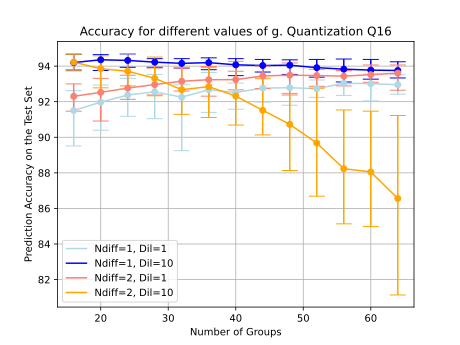
\includegraphics[width=0.75\textwidth]{fig/score_vs_g_q16.pdf}
    \caption{Accuracy of NanoHydra for the ECG5000 dataset across different values of $g$, input quantized in 16-bit. Four topologies considered, in increasing complexity, listed in the legend.}
    \label{fig:vs_g_q16}
\end{figure}
\begin{figure}[h!]
    \centerfloat
    \includegraphics[width=0.75\textwidth]{fig/score_vs_g_q8.pdf}
    \caption{Accuracy of NanoHydra for the ECG5000 dataset across different values of $g$, input quantized in 8-bit. Four topologies considered, in increasing complexity, listed in the legend.}
    \label{fig:vs_g_q16}
\end{figure}
\begin{figure}[h!]
    \centerfloat
    \includegraphics[width=0.75\textwidth]{fig/score_vs_dil_q16.pdf}
    \caption{Accuracy of NanoHydra for the ECG5000 dataset across different dilation levels $N\sb{\text{dil}}$, input quantized in 16-bit. Four topologies considered, in increasing complexity, listed in the legend.}
    \label{fig:vs_g_q16}
\end{figure}
\begin{figure}[h!]
    \centerfloat
    \includegraphics[width=0.75\textwidth]{fig/score_vs_dil_q8.pdf}
    \caption{Accuracy of NanoHydra for the ECG5000 dataset across different dilation levels $N\sb{\text{dil}}$, input quantized in 8-bit. Four topologies considered, in increasing complexity, listed in the legend.}
    \label{fig:vs_g_q16}
\end{figure}


\subsection{GAP9 Measurements}\label{sec:rs_gap9_meas}
To be done.

\begin{table}[h!]
    \centerfloat
    \rowcolors{2}{lightgray}{white}
    \begin{tabular}{ c c c c c c c }
    \toprule
    \textbf{Configuration Name} & $N\sb{\text{diff}}$ & \textbf{Kernels Per Group} & \textbf{Groups} & $N\sb{\text{dil}}$ \\
    \midrule
    CFGA & 1 & 8 & 16 & 3 \\
    CFGB & 2 & 8 & 16 & 5 \\
    \bottomrule
    \end{tabular}
    \caption{NanoHydra configurations used on the ECG5000 dataset tests on the GAP9}%
    \label{tbl:gap9_test_cfg}
\end{table}

\begin{table}[h!]
    \centerfloat
    \rowcolors{2}{lightgray}{white}
    \begin{tabular}{ c c c c }
    \toprule
    \textbf{Configuration Name} & Kernels (Step 1) & Classifier (Step 2 \& 3) & Activations \\
    \midrule
    CFGA & 0.070 kB &  3 kB & 0.75 kB \\
    CFGB & 0.070 kB & 10 kB & 2.5  kB \\
    \bottomrule
    \end{tabular}
    \caption{Memory requirements for the trainable parameters and activations in the different configurations of NanoHydra, in kB}%
    \label{tbl:gap9_test_cfg_reqmem}
\end{table}

\begin{table}[h!]
    \centerfloat
    \rowcolors{2}{lightgray}{white}
    \begin{tabular}{ c c c }
    \toprule
    \textbf{Configuration Name} & Kernels (Step 1) & Classifier (Step 2 \& 3)\\
    \midrule
    CFGA & 2.88  & 0.0064 \\
    CFGB & 0.864 & 0.00192 \\
    \bottomrule
    \end{tabular}
    \caption{Computational requirements for the trainable parameters and activations in the different configurations of NanoHydra, in MMACs}%
    \label{tbl:gap9_test_cfg_reqcomp}
\end{table}

\begin{table}[h!]
    \centerfloat
    \rowcolors{2}{lightgray}{white}
    \begin{tabular}{ c c c c c c c c}
    \toprule
    \textbf{Quantz.} & \textbf{Config} & \textbf{Parallel} & \textbf{Accuracy} & \textbf{MCycles} & \textbf{Inf. Time} & \textbf{Inf. Energy} & \textbf{Train Time} \\
    \midrule
    Q16 & CFGA & Yes & 94.38\% & 0.1312 & 1.312 ms & t.b.d. & 38 s\\
    Q16 & CFGB & Yes & 94.67\% & 0.4184 & 4.189 ms & t.b.d. & 95 s\\
    Q8  & CFGA & Yes & 94.13\% & 0.0956 & 0.956 ms & t.b.d. & 38 s\\
    Q8  & CFGB & Yes & 94.47\% & 0.2990 & 2.990 ms & t.b.d. & 95 s\\
    Q16 & CFGA & No  & 94.38\% & 0.7162 & 7.162 ms & t.b.d. & 38 s\\
    Q8  & CFGB & No  & 94.13\% & 0.4823 & 4.823 ms & t.b.d. & 38 s\\
    \bottomrule
    \end{tabular}
    \caption{Inference Results of the ECG5000 dataset on the GAP9. Results presented correspond to the average of 20 training/inference rounds. The reported accuracy is the maximum across these rounds, the train time is the total time of all 20 training rounds.}%
    \label{tbl:gap9_inf_results}
\end{table}

\newpage
\subsection{Comparison to Related Work}

\section{Proposal for Speech Commands Dataset}\label{sec:rs_speechcomms}
To be done.

\subsection{Comparison to Related Work}
\begin{table}
\begin{tabular}{||c|c|c|c|c|c|r|r||}
    \hline
    Reference & Model & TestAC & Memory & Ops & Year & Citation & Reproducible? \\

    \hline\hline
    \cite{Zhang2017}   &        DS-CNN & 94.4\% & 38.6 kB & 5.4M & 2017 & 483 &  \href{https://github.com/ARM-software/ML-KWS-for-MCU}{Yes} \\
    \cite{Andrade2018} &       Att-RNN & 96.9\% &  202 kB &   ?? & 2018 & 113 &  No \\
    \cite{Tang2018}    &       ResNet8 & 94.1\% &  110 kB &  30M & 2018 & 241 &  \href{https://github.com/castorini/honk/}{Yes} \\
    \cite{Tang2018}    & ResNet-Narrow & 90.1\% & 19.9 kB & 5.7M & 2018 & 241 &  \href{https://github.com/castorini/honk/}{Yes} \\
    \cite{Jansson2018} &    ConvNetRaw & 89.4\% &  700 kB &   5M & 2018 &  19 &  No \\
    \textbf{Ours}      &     NanoHydra & 88.7\% & 56.1 kB & 2.6M & 2024 & n/a &  Yes \\
    \hline
\end{tabular}
\end{table}

%\section{Current limitations}
%
%Demonstrating that your implementation meets the objectives is usually done by showing a lower bound on a given figure of merit.
%Conversely, you should also illuminate the limitations of your implementation by showing upper bounds on these (or other appropriate) figures of merit.
%Critically examining your ideas and their implementation trying to find their limits is also part of your work!
